\documentclass[a4paper,12pt]{article}
\usepackage{fouriernc}

\usepackage{pgfplots}
    \pgfplotsset{
        compat=1.11,
    }
\usetikzlibrary{shapes,arrows}

\tikzstyle{box}=[minimum size = 0.1cm, rectangle, draw=black, fill=gray]

\begin{document}

% LESS OPTIMIZED VERSION Declarative

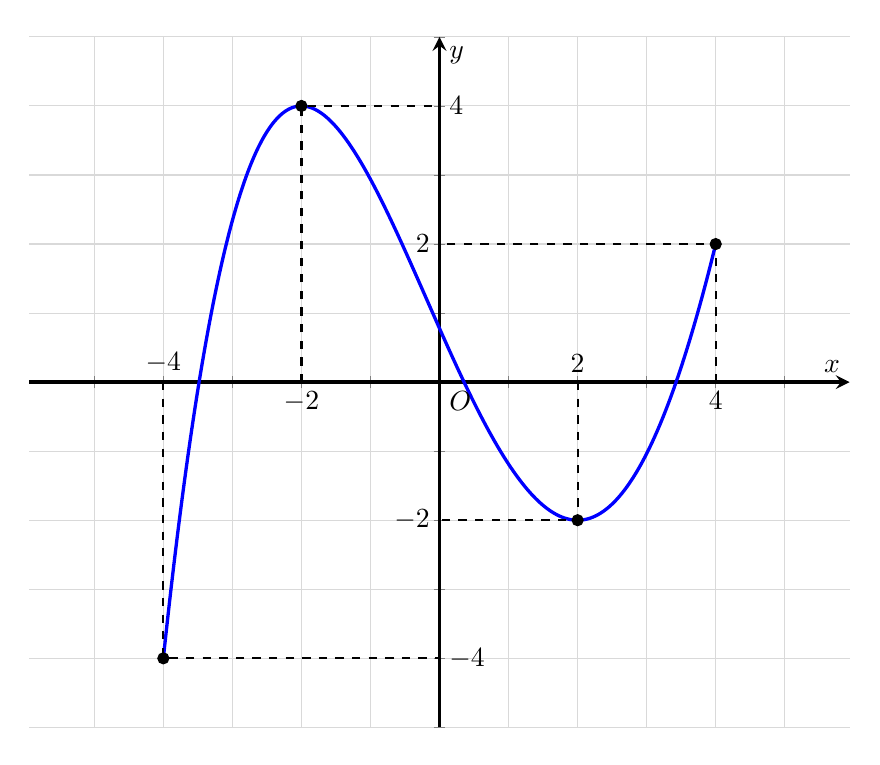
\begin{tikzpicture}[
    declare function={
        f(\x)=-(1/72)*\x^4+3/16*(\x^3)+(1/9)*\x^2-9/4*\x+7/9;
    }
    ]
    \begin{axis}[axis equal,
    width=12 cm, 
    grid=major, 
    axis x line=middle, axis y line=middle,
    axis line style = very thick,
    grid style={gray!30},
    ymin=-5, ymax=5, yticklabels={}, ylabel=$y$,
    xmin=-5, xmax=5, xticklabels={}, xlabel=$x$,
    samples=500,
    ]
    \addplot[blue, very thick,domain=-4:4, smooth]{f(x)};
    \node[below] at (-2, 0) {$-2$};
    \node[above ] at (-4, 0) {$-4$};
    \node[below ] at (4, 0) {$4$};
    \node[right] at (0,-4) {$-4$};
    \node[left  ] at (0,2) {$2$};
    \node[ right ] at (0,4) {$4$};
    \node[below right] at (0, 0) {$O$};
    \node[above ] at ( 2,0) {$2$};
    \node[left  ] at (0, -2) {$-2$};
    \addplot [mark=*,only marks,samples at={-4,-2,2,4}] {f(x)};
    ;
    \draw[dashed, thick] (-4,0) -- (-4,-4) -- (0,-4);
    \draw[dashed, thick] (-2,0) -- (-2,4) -- (0,4);
    \draw[dashed, thick] (2,0) -- (2,-2) -- (0,-2);
    \draw[dashed, thick] (4,0) -- (4,2) -- (0,2);
    \end{axis}
    \end{tikzpicture}

% MORE OPTIMIZED VERSION (with for each)

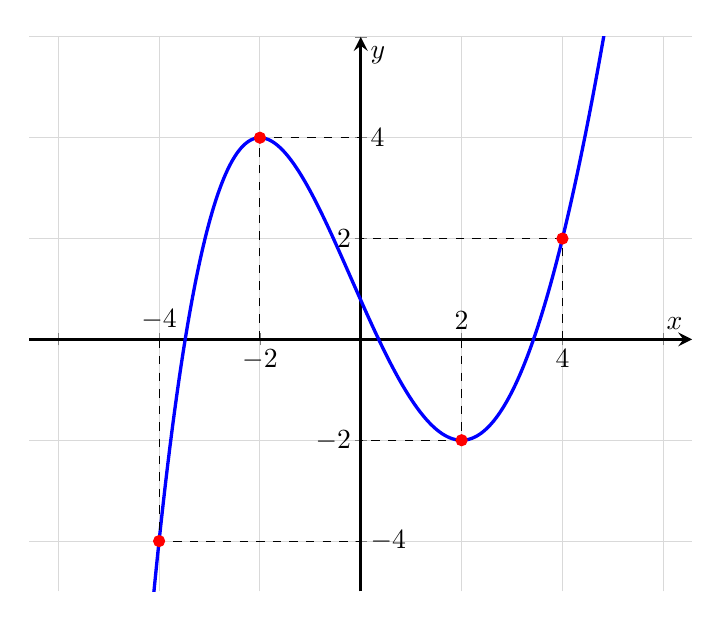
\begin{tikzpicture}[ 
declare function={ 
f(\x)=-(1/72)*\x^4+3/16*(\x^3)+(1/9)*\x^2-9/4*\x+7/9; 
} 
]
\begin{axis}[axis equal, 
width=10 cm, 
grid=major, 
axis x line=middle, axis y line=middle, 
axis line style = very thick, 
grid style={gray!30}, 
ymin=-5, ymax=6, yticklabels={}, ylabel=$y$, 
xmin=-4, xmax=4, xticklabels={}, xlabel=$x$, 
samples=500, 
] 
\addplot[blue, very thick,domain=-5:5, smooth]{f(x)}; 
\addplot [color=red, mark=*,only marks,samples at={-4,-2,2,4}] {f(x)}; 
\pgfplotsinvokeforeach{-4,-2,2,4}{\draw[dashed] ({#1},0) |- (0,{f(#1)}); }
\foreach \X/\Y in {-4/right,-2/left,2/left,4/right} 
{\edef\temp{\noexpand\node[\Y] at (0,\X) {$\X$};} 
\temp}
\foreach \X/\Y in {-4/above,-2/below,2/above,4/below} 
{\edef\temp{\noexpand\node[\Y] at (\X,0) {$\X$};} 
    \temp} 
\end{axis}
\end{tikzpicture}



\end{document}
